\section{Fine tuning a network machine learning model}
\label{sec:ch2:finetune}

Now that you have figured out an appropriate way to represent your network to learn from it, and you have learned how to train an algorithm to learn from it, it's time to tune things up a little bit.

In the last section, you learned how you can take one of the networks, and use embeddings combined with various clustering techniques to learn about latent structure in your data.

However, there's a big caveat: your colleague sent you over a hundred networks, and you ignored all but one of them! Surely, there's something that you can learn from all of them, right?

Fortunately, when you have a multiple network problem, there are plenty of approaches that you can use to learn from all of them simultaneously. Let's break down how we can approach this now.

So, you know that you want to produce a representation of all of your networks. These networks all have the same nodes, which are the different areas of the brain. For all intents and purposes, you can assume that these different nodes mean the same thing across all of the different people, even if they are different based on each individual. What you want to learn is whether there is some {shared} structure across all of the different networks present in the nodes. To do this, you are going to want to be able to take {all} of your networks, and produce an embedding in which you can look at each {node} as its own object. Does anything exist to help you?

There sure does. As you will learn, a particular representation called \texttt{MASE} from Section \ref{ch6:multinet:mase} does just this. It allows you to take many networks, and learn a single representation for the nodes across all of the networks. This representation, in particular, is going to effectively {borrow strength} from all of the networks you pass in, so you won't have to worry about whether you are just ignoring all of the networks but one like you did before. Let's see what \texttt{MASE} can do for us here:


\begin{lstlisting}[style=python]
from graspologic.embed import MultipleASE

embedding = MultipleASE().fit_transform(As)
_ = pairplot(embedding, title="Multiple spectral embedding of all connectomes")
\end{lstlisting}

Let's take a look at what happens when we apply our clustering to this embedding instead:

\begin{lstlisting}[style=python]
labels = AutoGMMCluster(max_components=10).fit_predict(embedding)
_ = pairplot(embedding, labels=labels,
                title="Multiple spectral embedding of all connectomes", 
                legend_name="Predicted Clusters")
\end{lstlisting}
The pairs plot of the \texttt{MASE} embedding with labels estimated by \texttt{GMM} is shown in Figure \ref{fig:ch2:mase}. Again, the clustering algorithm applied has some element of randomness to it, so don't be concerned if you don't get the exact same number of predicted clusters as we did, or if your clusters look a little different.

\begin{figure}[h]
    \centering
    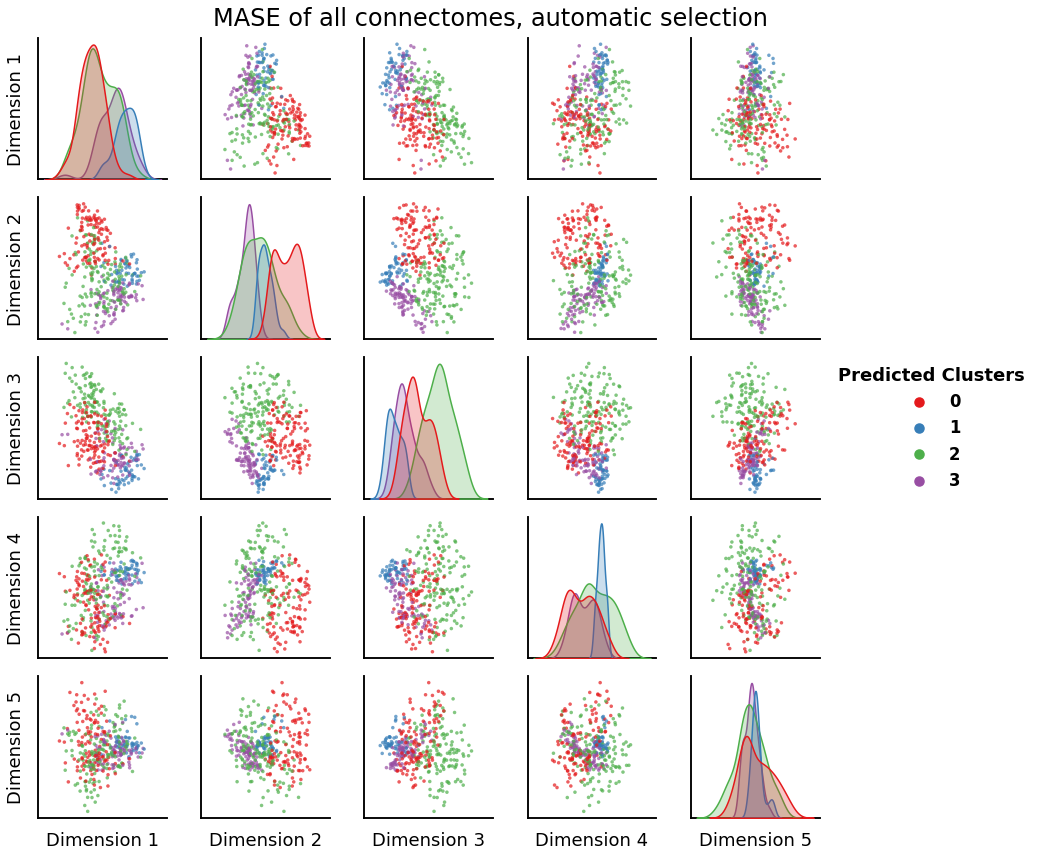
\includegraphics[width=\linewidth]{foundations/ch2/Images/mase.png}
    \caption[Joint embedding with estimated labels for connectomes]{\textbf{(A)} The \texttt{MASE} embedding, which learns an embedding across all networks in your dataset. \textbf{(B)} The \texttt{MASE} embedding, with labels learned by \texttt{GMM}.}
    \label{fig:ch2:mase}
\end{figure}
\newpage